\section{Introduction}\label{introduction}

Sample citation of \citet{Richardson1922}.

The atmosphere is in motion and it is a continuous mixing and clashing
of vortices and structures, but when it is averaged over a long period
of time (\fig{\ref{fig:ERA5-wind200}}) it shows a remarkable simple structure.
The figure shows the wind at an approximate level of about 12km, that is
considered to be in the free atmosphere, far from the influence of the
ground. The circulation is a large vortex around the pole that shows
small oscillation in latitudes, especially pronounced over North America
and the Asian Pacific Coast. The flow is therefore predominantly in the
East-West direction, with a relatively small component in the meridional
direction. The \emph{circumpolar vortex} has been one of the first
structures to be recognized when plentiful observations of the upper air
flow became available, but it provided some of the intriguing questions
that drove the development of geophysical fluid dynamics to this time.
some of them have not been completely understood. What is maintaining
this peculiar circulation ? Which factor determines the amplitude and
location of the undulations in meridional direction ? Some of these
question will be addressed in these notes

\begin{figure}
\centering
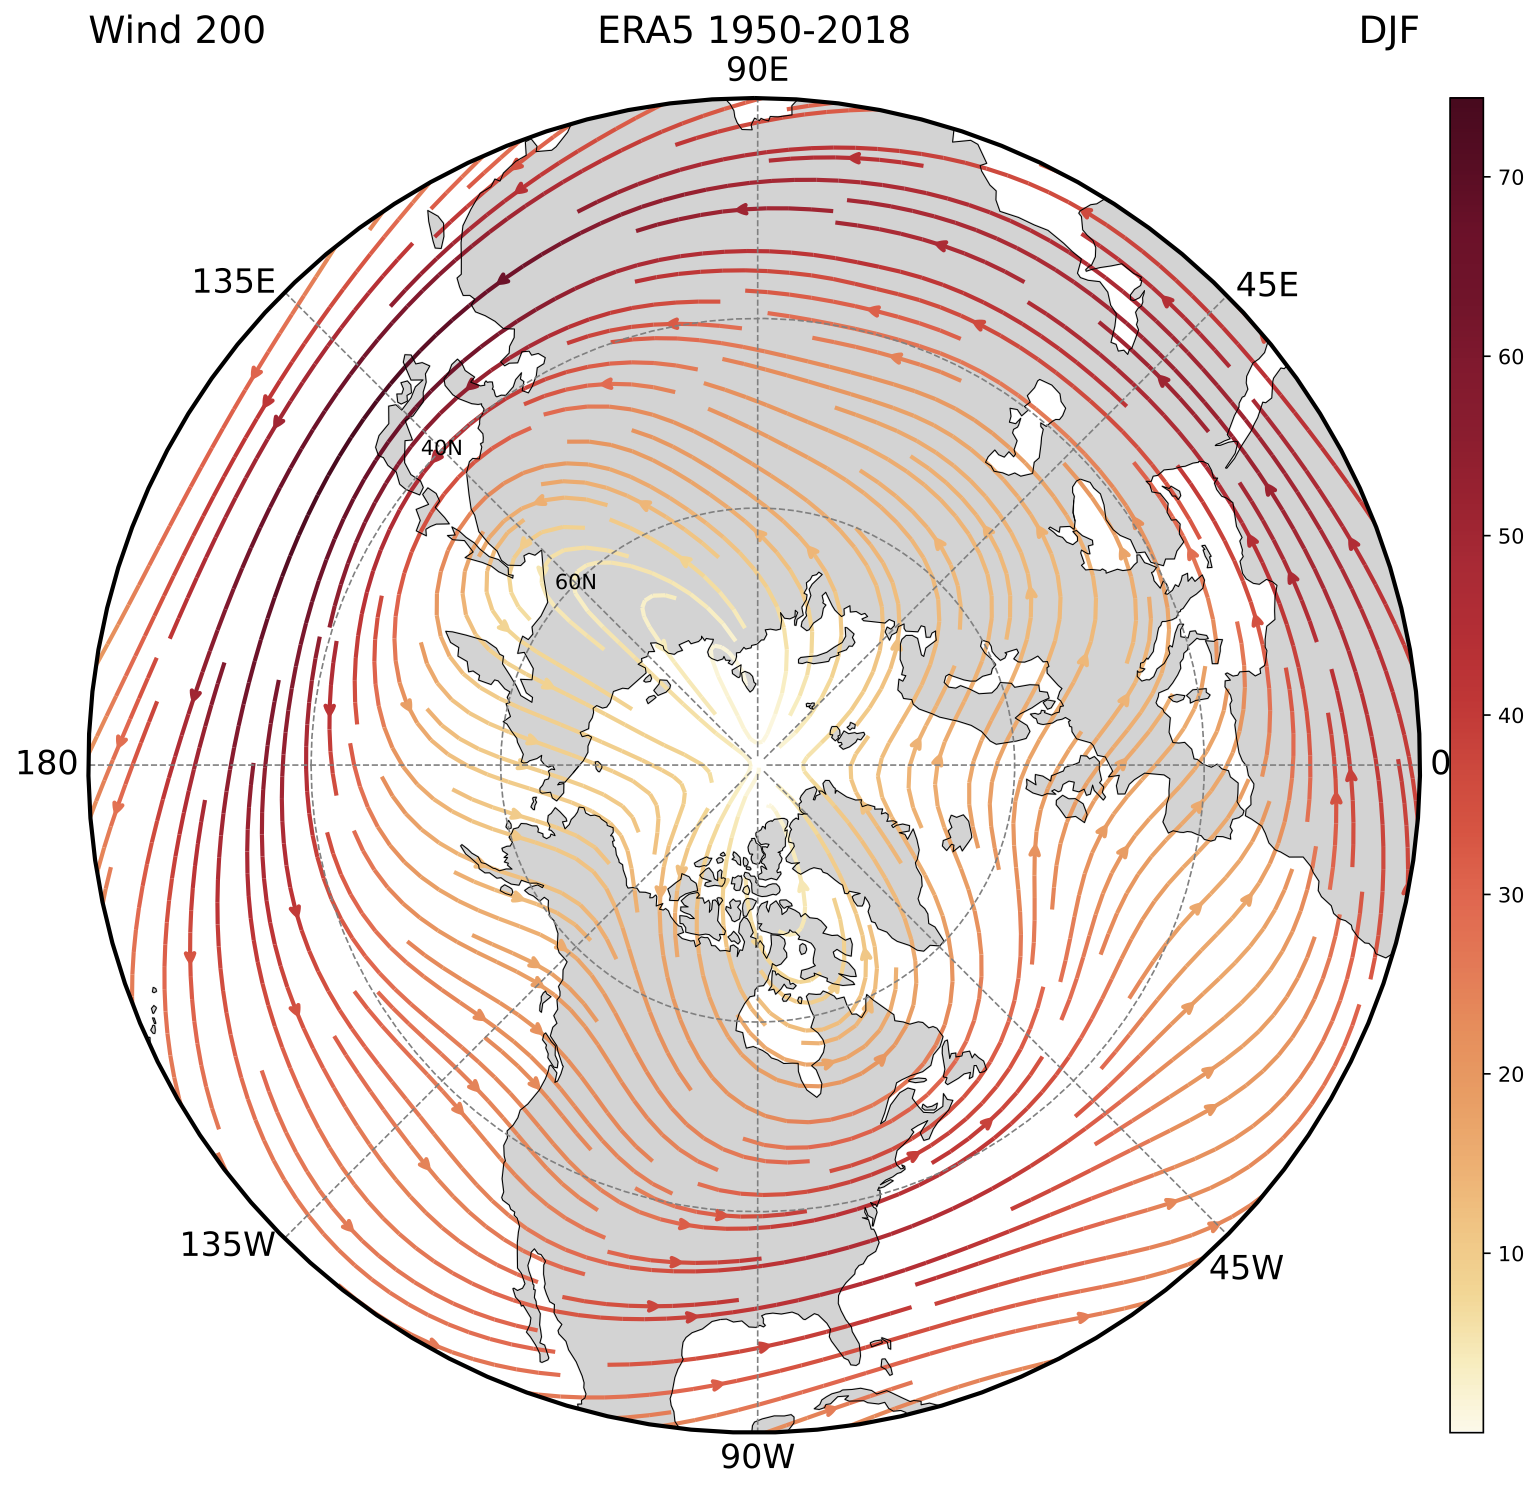
\includegraphics[width = .7 \textwidth]{figs/GD/Wind200.png}
\caption{}
\label{fig:ERA5-wind200}
\end{figure}


\subsection{Coordinate systems}\label{coordinate-systems}

\subsubsection{Spherical Coordinates}\label{spherical-coordinates}

The most commonly used coordinate system for the analysis of the
atmosphere and the oceans is a spherical coordinate system attached to
the rotating Earth (Fig. \texttt{fig:0} ). The spherical coordinates are
slightly different from the usual mathematical ones as the latitude is
measured from the equator and therefore it can take negative values. The
longitude is running west to east.

The longitude is also known as the ``zonal'' direction whereas the
latitude is also known as the "meridional" direction. Winds are
identified by the direction they are coming from, so a "westerly" wind
is coming \emph{from} the West and an "easterly" wind is coming from the
East.

This coordinate system is rotating with the Earth and therefore it
generates force terms in any dynamical equation expressed in this system
of coordinate, the Coriolis terms.

\begin{figure}
\centering
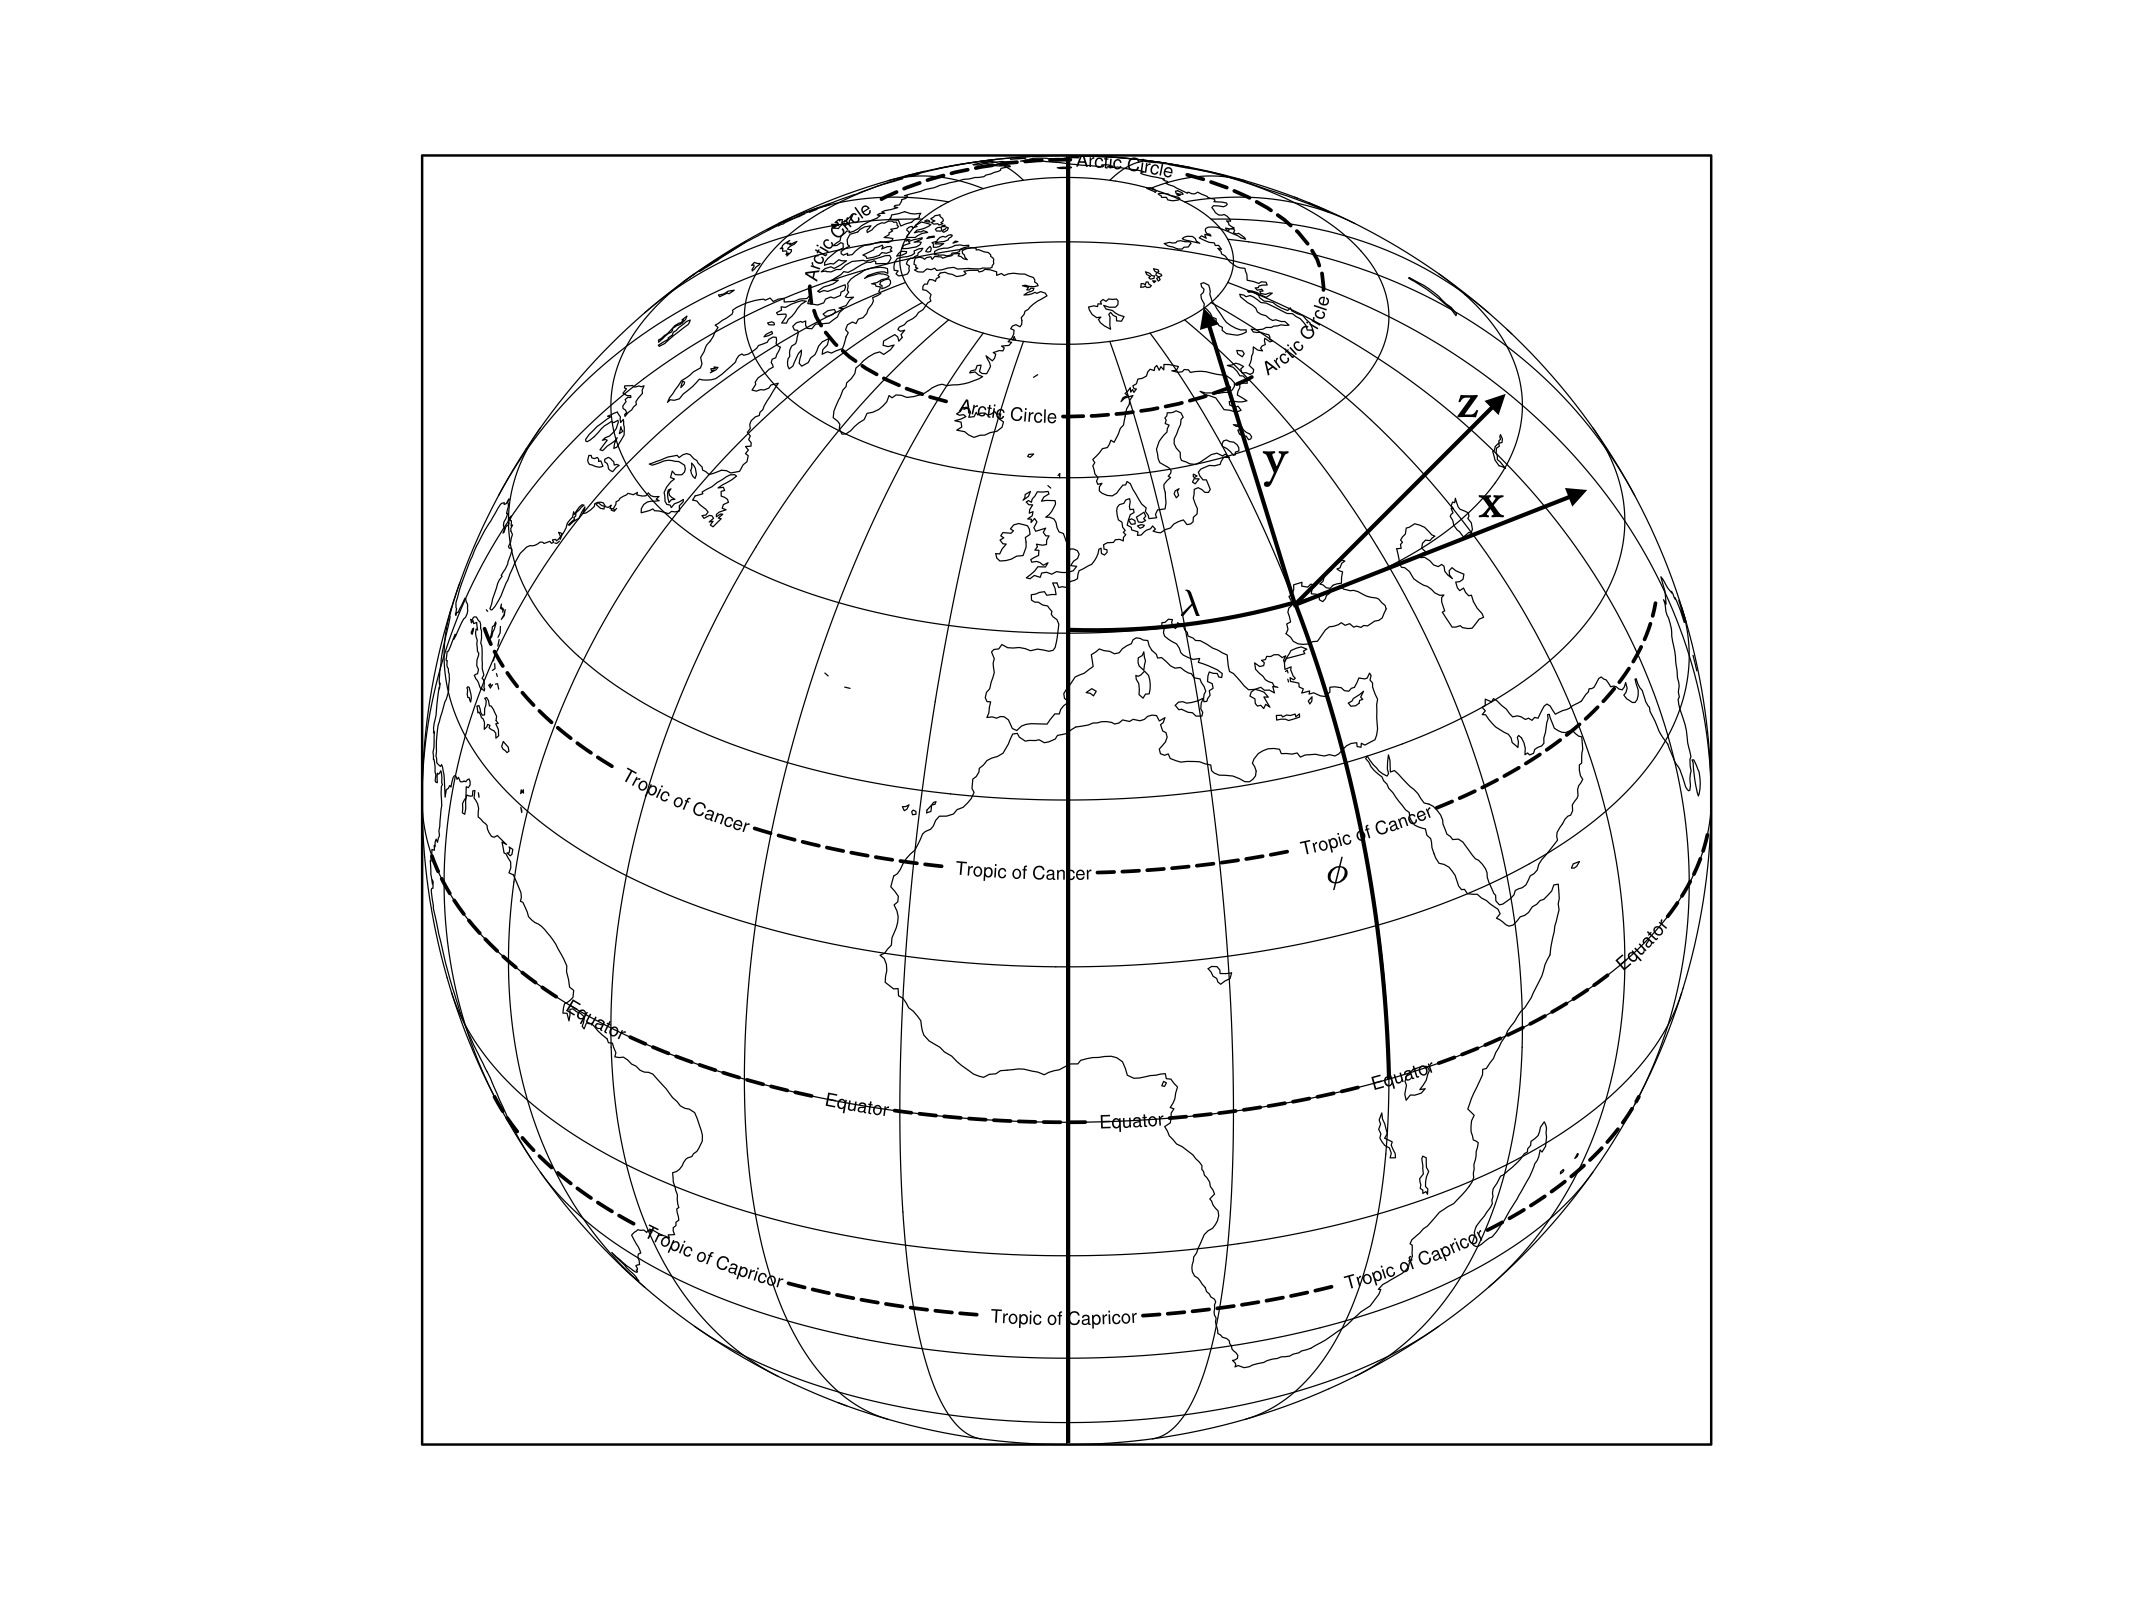
\includegraphics[width = .7 \textwidth]{figs/GD/map.png}
\caption{Coordinate System}
\label{fig:3d-coordinate-system}
\end{figure}

\subsubsection{The Beta-plane}\label{the-beta-plane}

It is sometimes convenient to shift coordinate system if the latitudinal
extension of the motion is not too great with respect to the motion
parameters as they are expressed in the adimensional numbers. When this
is possible, a tangent coordinate system is applied at a specific
latitude \(\phi_0\) and the resultant Cartesian coordinates system is
called the \(\beta\)-plane. Usually symbols \((x,y)\) are used in this
case for the zonal and meridional coordinate. In the \(\beta\)-plane the
planetary vorticity \(f\) is linearized as \(f=f_0 + \beta y\), where
\(\beta = \frac{\partial f}{\partial y}({\phi_0})\).

\subsection{Advective derivative}\label{Sec:Adv}

To describe the governing equation of the atmosphere and eventually of
the ocean we have to understand how we write the rate of change with
time of this fluid. This problem was solved by considering the fact that
the rate of change in the fluid cannot be seen as arate of change with
respect to a fixed system of coordinate because the system is moving
with the fluid itself. Therefore, first we have to find a way to
describe the change taking into account the moving system of
restaurants. These can be done by using a concept developed in the 19th
century by Euler that is called "advective derivative" that can be
obtained from a total derivative of the property,

\[\frac{d \phi}{dt} = \frac{\partial \phi}{\partial t} + \frac{\partial x}{\partial t}\frac{\partial \phi}{\partial x} + \frac{\partial y}{\partial t}\frac{\partial \phi}{\partial y}+\frac{\partial z}{\partial t}\frac{\partial \phi}{\partial z} = \frac{\partial \phi}{\partial t} + \mathbf{v}\cdot\nabla\phi\]

and so it can be defined as

\[\frac{D \varphi}{Dt} =\frac{\partial \varphi}{\partial t} + \mathbf{v}\cdot\nabla\varphi\]

in this way the moving fluid can be described by derivatives with
respect the "fixed" coordinate system, i.e. the Eulerian description.
The alternative description of the observer moving with fluid is known
as the "Lagrangian" description.

\subsection{Primitive Equations}\label{Sec:Prim}

The equation governing the motion of the atmosphere can be written as:

\[\begin{aligned}
&\frac{D u}{Dt} -\frac{uv \tan{\phi}}{r} +  \frac{uw}{r} = -\frac{1}{\rho r \cos{\phi}}\frac{\partial p}{\partial \lambda} + fv - \hat{f}w + F_\lambda\\
&\frac{D v}{Dt} -\frac{u^2 \tan{\phi}}{r} +  \frac{vw}{r} = -\frac{1}{\rho r }\frac{\partial p}{\partial \phi} - fu  + F_\phi\\
&\frac{D w}{Dt} -\frac{u^2+v^2}{r} = -\frac{1}{\rho }\frac{\partial p}{\partial z} -g +\hat{f}u + F_z\\
\end{aligned}\]

the \(f=2\Omega \sin{\phi}\) and \(\hat{f} = 2\Omega\cos{\phi}\) terms
arise from the rotating spherical coordinate system that we have chosen,
other terms are generated by the spherical geometry. Some of them are
small and traditionally they can be neglected, so that we arrive at the
system

\[\begin{aligned}
&\frac{D u}{Dt} - v\left(f +  \frac{u \tan{\phi}}{a}\right)  = -\frac{1}{\rho a \cos{\phi}}\frac{\partial p}{\partial \lambda}   + F_\lambda\\
&\frac{D v}{Dt} + u\left( f + \frac{u \tan{\phi}}{a}\right)  = -\frac{1}{\rho a}\frac{\partial p}{\partial \phi}  + F_\phi\\
&\frac{D w}{Dt}  = -\frac{1}{\rho }\frac{\partial p}{\partial z} -g  + F_z\\
\end{aligned}\]

where we have also used the \emph{Shallowness Approximation} by assuming
\(r = a +z \approx a\), where \(a\) is the Earth radius.

However the advective derivative must be expressed in spherical
cordinates

\[\frac{D }{Dt} = \frac{\partial }{\partial t} + \frac{u}{a\cos{\phi}}\frac{\partial }{\partial \lambda} +\frac{v}{a}\frac{\partial }{\partial \phi} + w\frac{\partial }{\partial z}\]

so that the velocity components are

\[\begin{aligned}
&u = a\cos{\phi\frac{\partial \lambda}{\partial t}}\\
&v = a \frac{\partial \phi}{\partial t}\\
&w = \frac{\partial z}{\partial t}
\end{aligned}\]

These equation govern the mechanical behaviour of the atmosphere, and we
will see in a different form, also of the ocean. There three forces in
action: pressure gradient, rotaiton via the Coriolis force and gravity.

The equation are not complete,we have three equation but five variables,
so we need to find the missing relations. We are using the basic
conservation principles, the latter equations describe the conservation
of momentum, we can exploit the conservation of mass. The mass of the
fluid must be conserved locally, because there are now sinks or sources
in the atmosphere itself, so we want to write the mass of a volume of
atmosphere fixed in space as
\[M = \int_V  \rho \,dV\]
the mass in the volume can only change if there is a flux of mass at
surface \(S\),
\[\frac{\partial }{\partial t} \int_V  \rho \,dV = -\int_S \rho\mathbf{v}\cdot n \, dS\]
using the divergence theorem however we have
\[\frac{\partial }{\partial t} \int_V  \rho \,dV = -\int_V \nabla\cdot(\rho\mathbf{v}) \,dV\]
because the volume is not changing with time we can bring the derivative
inside the integral and we get
\[\int_V  \frac{\partial \rho}{\partial t}+\nabla\cdot(\rho\mathbf{v}) \,dV = 0\]
but the volume is arbitrary, so it must be that
\[\frac{\partial \rho}{\partial t}+\nabla\cdot(\rho\mathbf{v}) = 0\]

is valid locally.

We have still at our disposal the conservation of thermodynamical energy
and so we can also use

\[C_v\frac{D T}{Dt} = -p\frac{D }{Dt}\left(\frac{1}{\rho}\right)+ Q\]

where we included the temperature and heating/cooling term \(Q\). The
state variable are then linked by the state equation

\[p = \rho R T\]

where \(R\) is the gas constant for dry air.

We can use the equation of state to write the energy equation ( or the
temperature equation) in a different form,

\[c_v\frac{D T}{Dt} = -p\frac{D }{Dt}\left(\frac{R T}{p}\right)+ Q = -R\frac{D T}{Dt} + \frac{RT}{p}\frac{D p}{Dt} + Q\]

yielding the alternative forms ( since \(c_p = c_v +R\)),

\[c_p\frac{D T}{Dt}  - \frac{1}{\rho}\frac{D p}{Dt} = Q\]

For adiabatic processes \(Q=0\) and so

\[\begin{aligned}
&c_p\frac{D T}{Dt}  - \frac{1}{\rho}\frac{D p}{Dt} = 0\\
&\frac{c_p}{T}\frac{D T}{Dt} -\frac{R}{p}\frac{D p}{Dt} = 0\\
&\frac{D }{Dt}\log{T} - \frac{R}{c_p}\frac{D }{Dt}\log{p} = 0
\end{aligned}\]

integrating it we get

\[\log{T/T_0} - \log{\left(\frac{p}{p_0}\right)^{R/c_p}} = const\]

or

\[\frac{T}{T_0}\left(\frac{p_0}{p}\right)^{R/c_p} = const\]

so the quantity, known as \emph{potential temperature}

\[\theta = T\left(\frac{p_0}{p}\right)^{R/c_p}\]

is conserved in adiabatic processes and the thermodynamics equation can
be written as

\[\frac{D \theta}{Dt} = Q\]

\subsection{Hydrostatic balance}\label{hydrostatic-balance}

Under the action of gravity the vertical component of the pressure
gradient force balances the action of gravity, resulting in very small
vertical acceleration

\[\frac{\partial p}{\partial z} =  -g \rho\]

then if we take the vertical derivative of the eq. \texttt{Eq:logT}

\[\frac{1}{T_0}\frac{d T}{dz}\left(\frac{p_0}{p}\right)^{R/c_p} -\frac{p_0}{p^2}\frac{R}{c_p}\frac{T}{T_0}\left(\frac{p_0}{p}\right)^{R/c_p-1}\frac{d p}{dz} = 0\]

simplifying

\[\frac{d T}{dz} -\frac{p_0}{p^2}\frac{R}{c_p}T\left(\frac{p_0}{p}\right)^{-1}\frac{d p}{dz} = 0\]

or

\[\frac{d T}{dz} -\frac{1}{p}\frac{R}{c_p}T\frac{d p}{dz} = \frac{d T}{dz} +g\rho\frac{1}{p}\frac{R}{c_p}T = 0\]

but using the equation of state

\[\frac{d T}{dz} = -\frac{g}{c_p}\]

that gives how the temperature change with height under adiabatic
conditions and when the hydrostatic balance is valid. This is known as
the \emph{adiabatic lapse rate}.

\subsection{Summary of fundamental
equations}\label{summary-of-fundamental-equations}

Summarizing our discussion, the fundamental equation that describe the
motion of the atmosphere then are:

\[\begin{aligned}
&\frac{D u}{Dt} - v\left(f +  \frac{u \tan{\phi}}{a}\right)  = -\frac{1}{ a \cos{\phi}}\frac{1}{\rho}\frac{\partial p}{\partial \lambda}   + F_\lambda \\
&\frac{D v}{Dt} + u\left( f + \frac{u \tan{\phi}}{a}\right)  = -\frac{1}{a}\frac{1}{\rho}\frac{\partial p}{\partial \phi}  + F_\phi \\
&\frac{D w}{Dt}  = -\frac{1}{\rho }\frac{\partial p}{\partial z} -g  + F_z \label{Eq:PrimEq}\\
&\frac{D \theta}{Dt} = Q \\
&\frac{\partial \rho}{\partial t}+\frac{1}{a\cos{\phi}}\left[ \frac{\partial }{\partial \lambda}(\rho u) + \frac{\partial }{\partial \phi}(rv\cos{\phi} \right] +\frac{\partial }{\partial z}(\rho w) = 0 \\
&p = \rho R T
\end{aligned}\]

where we have used the divergence in spherical coordinates.

These equations are still not closed because we will need to express the
heating/cooling term \(Q\) and the friction terms \(F\) as a function of
the state variables. This will require a theory of the processes that
drive them. Where \(R=287.052874 J \quad kg^{-1} K^{-1}\) is the gas
constant for dry air and \(c_p = 1.005\) is the specific heat at
constant pressure, \(c_v = 0.718\) is the specific heat at constant
volume, \(\kappa = \frac{R}{c_p}\) and \(\gamma=c_p/c_v\) is their
ratio.

For theoretical and idealized studies the set of equation projected on
the \(\beta\)-plane is also used

\[\begin{aligned}
&\frac{D u}{Dt} - fv  = -\frac{1}{\rho}\frac{\partial p}{\partial x}   + F_x \\
&\frac{D v}{Dt} + fu = -\frac{1}{\rho}\frac{\partial p}{\partial y}  + F_y \\
&\frac{D w}{Dt}  = -\frac{1}{\rho }\frac{\partial p}{\partial z} -g  + F_z \\
&\frac{D \theta}{Dt} = Q\\
&\frac{\partial \rho}{\partial t}+\nabla\cdot(\rho\mathbf{v}) = 0\\
&p = \rho R T
\end{aligned}\]

and the gradient operator is the cartesian operator

\[\nabla = \frac{\partial }{\partial x} + \frac{\partial }{\partial y} + \frac{\partial }{\partial z}\]

and the advective derivative is then

\[\frac{D }{Dt} = \frac{\partial }{\partial t} + u\frac{\partial }{\partial x} + v\frac{\partial }{\partial y} + w\frac{\partial }{\partial z}\]
